% main tex file

% begin ACM TAPS stuff
\documentclass[sigconf,review,anonymous]{acmart}

%%
%% \BibTeX command to typeset BibTeX logo in the docs
\AtBeginDocument{%
  \providecommand\BibTeX{{%
    \normalfont B\kern-0.5em{\scshape i\kern-0.25em b}\kern-0.8em\TeX}}}

%% Rights management information.  This information is sent to you
%% when you complete the rights form.  These commands have SAMPLE
%% values in them; it is your responsibility as an author to replace
%% the commands and values with those provided to you when you
%% complete the rights form.
\setcopyright{acmcopyright}
\copyrightyear{2018}
\acmYear{2018}
\acmDOI{XXXXXXX.XXXXXXX}

%% These commands are for a PROCEEDINGS abstract or paper.
\acmConference[Conference acronym 'XX]{Make sure to enter the correct
  conference title from your rights confirmation emai}{June 03--05,
  2018}{Woodstock, NY}
\acmPrice{15.00}
\acmISBN{978-1-4503-XXXX-X/18/06}

% end ACM TAPS stuff

% my own stuff
\usepackage{xac}

\begin{document}

\title{AwesomePaper: This is an Awesome HCI Paper}

%%
%% By default, the full list of authors will be used in the page
%% headers. Often, this list is too long, and will overlap
%% other information printed in the page headers. This command allows
%% the author to define a more concise list
%% of authors' names for this purpose.
\renewcommand{\shortauthors}{Trovato and Tobin, et al.}

%%
%% The abstract is a short summary of the work to be presented in the
%% article.
\begin{abstract}
  \input{00_abstract}
\end{abstract}


\ccsdesc[500]{Human-centered computing~Interactive systems and tools}

%%
%% Keywords. The author(s) should pick words that accurately describe
%% the work being presented. Separate the keywords with commas.
\keywords{keyword1, keyword2, keyword3, keyword4}

%% A "teaser" image appears between the author and affiliation
%% information and the body of the document, and typically spans the
%% page.
\begin{teaserfigure}
  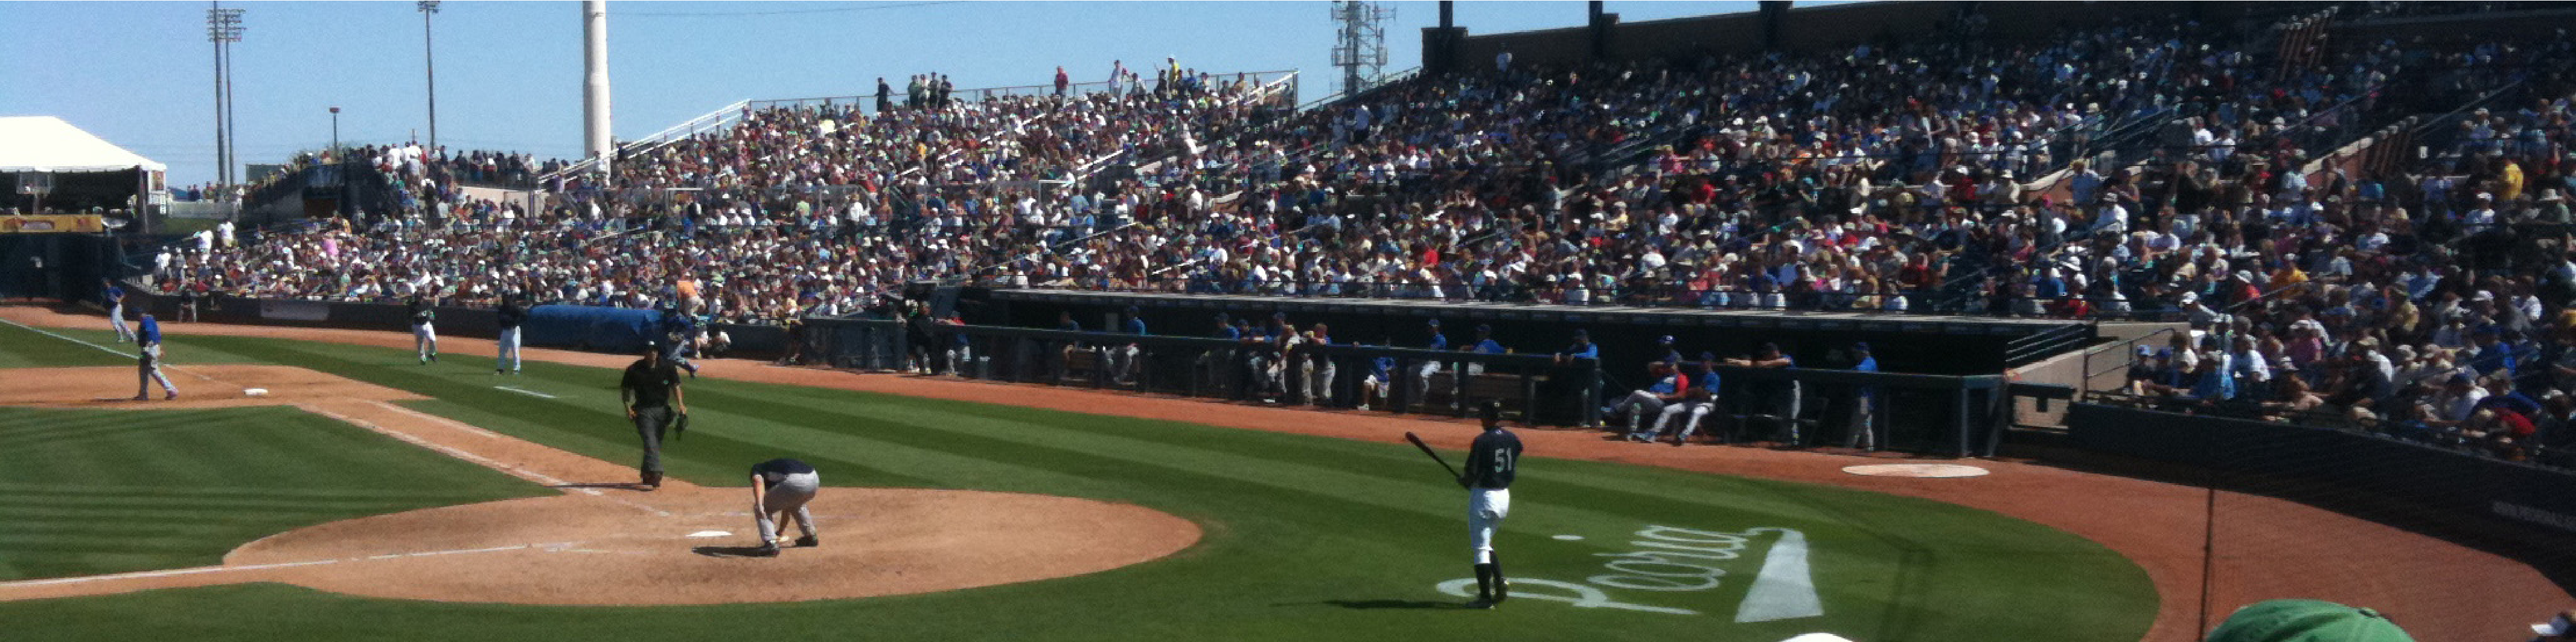
\includegraphics[width=\textwidth]{figures/sampleteaser}
  \caption{Seattle Mariners at Spring Training, 2010.}
  \Description{Enjoying the baseball game from the third-base
  seats. Ichiro Suzuki preparing to bat.}
  \label{fig:teaser}
\end{teaserfigure}

%%
%% This command processes the author and affiliation and title
%% information and builds the first part of the formatted document.
\maketitle

\section{Introduction}

% PROMISE: What is a technology that promises us something good?
The recent development of \xx promises to [make the world a better place] \xxx

% PROBLEM: What is the problem that prevents this technology from realizing its promise?
However, the problem is \xxx

% PRIOR WORK: What is the most representative prior work that has attempted to solve this problem and why did it fail?
To solve this problem, past work has \xxx

% PROPOSED SOLUTION: What is your proposed solution given where prior work fell short?
To fill in this gap, we design and implement \xxx
% Use an example (and refer to figure 1) to walkthrough your research in more details
As shown in \fgref{fig1}, \xxx

% PROOF
% What is your proof to validate that your proposed solution contributes to solving that problem?
To validate \xx, we conducted \xxx

% CONTRIBUTION
{\bf The main contribution} of this paper is \xxx
% differentiate from prior work
In contrast to prior work that \xxx
\section{Related Work}
% briefly explain why your research is related to what you review below
Our research focuses on \xxx, which is related to \xxx

\subsection{[related work area \#1]}

\subsection{[related work area \#2]}

\subsection{[related work area \#3]}
\section{Formative Study}
\section{Design}
\section{Implementation}
\section{User Study}
\section{Discussions}
\section{Conclusion}

Remove this citation later: \cite{bush1945we}.

\bibliographystyle{ACM-Reference-Format}
\bibliography{ref_main}

\end{document}